\section{Conceptos previos}
En este apartado se describe la arquitectura de VMware Cloud Foundation, como estructura sus componentes internamente y cuales son los requisitos mínimos para realizar el despliegue de la plataforma\footnote{Se describen solo aquellos componentes que se utilizarán en el despliegue de Cloud Foundation.}.

%%%%%%%%%%%%%%%%%%%%%%%%%%%%%%
\iffalse
En este apartado se explican aquellos conceptos de VMware Cloud Foundation necesarios para entender su funcionamiento, configuración y requisitos de la infraestructura previos al despliegue del servicio.
\fi
%%%%%%%%%%%%%%%%%%%%%%%%%%%%%%%%


%% Workload Ddomains %&%&%%%%
%%%%%%%%%%%%%%%%%%%%%%%%%%%%
\subsection{Workload Domain}
Un \textit{workload domain} consiste en una abstracción lógica de una parte de la capacidad de la infraestructura para consumirla. Se extiende sobre varios hosts creando un cluster aparentemente aislado. Cada \textit{workload domain} tiene su propia instancia de vCenter Server, vSAN y NSX. Existen \underline{tres tipos} de \textit{workload domains} que permiten aislar las tareas de gestión de las tareas de los usuarios. 

%% MANAGEMENT DOMAIN
\subsubsection{Management Domain}
\label{subsubsec:domainManagement}
Este \textit{workload domain} se crea y configura automáticamente durante el proceso de despliegue de Cloud Foundation. Se dedicada a tareas de gestión de los componentes del entorno. Los componentes dedicados a este \textit{workload domain} son SDDC Manager, vCenter Server, dos Platform Services Controllers que son redundantes, vRealize Log Insight y un vSwitch Distributed.\\
Este dominio precisa estos \underline{requisitos mínimos de hardware}:
\begin{itemize}
    \item \textbf{Hosts}: 4
    \item \textbf{CPU} por host: Dual-socket con 8 cores por socket, en sistemas All-Flash.
    \item \textbf{Memoria} por host: 192 GB
    \item \textbf{Almacenamiento} por host: 16 GB para el dispositivo de arranque, un NVMe o SSD para la capa de caché, dos SSD o HDD para la capa de capacidad.
    \item \textbf{NICs} por host: Dos NICs de al menos 10 GbE y, opcionalmente un NIC 1GbE BMC.
\end{itemize}

Cuando se \underline{despliega Management Domain se crean y configuran} de forma automatizada por SDDC Manager las siguientes máquinas virtuales (VM) de cada componente de Cloud Foundation:
\begin{itemize}
    \item Una VM de \textbf{SDDC Manager}: 4 vCPU, 16 GB de memoria, 800 GB de almacenamiento.
    \item Una VM de \textbf{vCenter Server}: 4 vCPU, 16 GB de memoria, 290 GB de almacenamiento.
    \item Dos instancias de \textbf{Platform Services Controller} (cada una): 2 vCPU, 4 GB de memoria, 60 GB de almacenamiento.
    \item Una VM de \textbf{NSX Manager}: 4 vCPU, 16 GB de memoria, 60 GB de almacenamiento.
    \item Tres VM de \textbf{NSX Controller} (cada una): 4 vCPU, 4 GB de memoria, 28 GB de almacenamiento.
    \item Tres VM de \textbf{vRealize Log Insight}, una en cada nodo: 8 vCPU, 16 GB de memoria, 1312 GB de almacenamiento.
\end{itemize}


%% VIRTUAL INF. DOMAIN
\subsubsection{Virtual Infrastructure Domain (VI) y Virtual Desktop Infrastructure Domain (VDI)}
\label{subsubsec:domainVI}
Este \textit{workload domain} es creado manualmente por el administrador y en un mismo entorno pueden existir múltiples Virtual Infrastructure Domains. Las capacidades de este dominio se especifican durante su proceso de creación, pudiendo indicar el número de nodos sobre los que se despliega, cantidad de almacenamiento, tipo de rendimiento y tipo de disponibilidad para satisfacer las necesidades del usuario, el cual realizará sus tareas dentro de este \textit{workload domain}. El usuario accede a este dominio a través de vSphere Client donde puede editar la configuración de los hosts, aplicaciones y máquinas virtuales.
Cada Virtual Infrastructure Domain tiene un vCenter Server dedicado que se ejecuta desde Management Domain y su propio sistema vSAN y NSX.\\
La única diferencia de Virtual Desktop Infrastructure Domain es que este incorpora el producto VMware Horizon View que, resumiendo, permite desplegar escritorios virtuales.\\
El dominio VI precisa estos \underline{requisitos mínimos de hardware}:
\begin{itemize}
    \item \textbf{Hosts}: 3
    \item \textbf{CPU}, \textbf{Memoria} y \textbf{Almacenamiento}: depende de la configuración que se establezca.
    \item \textbf{NICs} por servidor: Dos NICs de al menos 10 GbE y, opcionalmente un NIC 1GbE BMC.
\end{itemize}

Cuando se \underline{despliega un VI Domain se crean y configuran} de forma automatizada por SDDC Manager las siguientes máquinas virtuales (VM) de cada componente de Cloud Foundation:
\begin{itemize}
    \item Una VM de \textbf{vCenter Server} en Management Domain: 8 vCPU, 24 GB de memoria, 500 GB de almacenamiento.
    \item Una VM de \textbf{NSX Manager} en Management Domain: 4 vCPU, 16 GB de memoria, 60 GB de almacenamiento.
    \item Tres VM de \textbf{NSX Controller} en el VI Domain creado (cada una):  4 vCPU, 4 GB de memoria, 28 GB de almacenamiento.
\end{itemize}

En total, si la infraestructura cuenta con un Management Domain y al menos un Virtual Infraestructure Domain, entonces se necesita una \setword{capacidad}{Word:capacidad} inicial y como mínimo igual a 76 vCPU, 168 GB de Memoria y 3306 GB de almacenamiento.

\begin{figure}[h!]
  \centering
  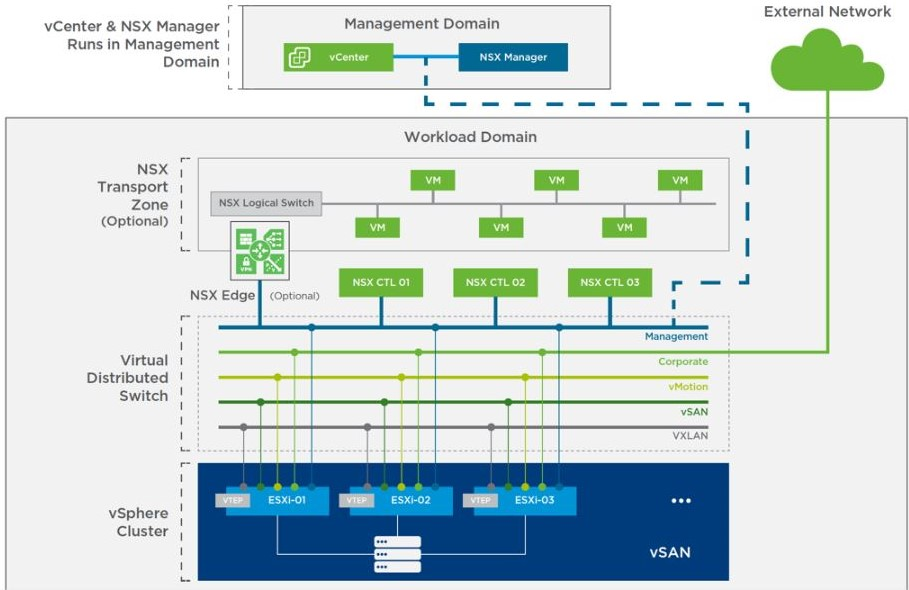
\includegraphics[width=1\textwidth]{imaxes/conceptosPrevios/WDomainStructure.JPG}
  \caption{Estructura de los componentes de Cloud Foundation y Workload Domains.}
  \label{fig:esquemaCFDominios}
\end{figure}

\FloatBarrier

%&%%%%%%%%%%%%%%%%%%%%%%%%%%%%%%%%%%%%%%%%%%%%%%%%%%%%%%%%
%% ARQUITECTURA
\subsection{Arquitectura}
La arquitectura de VMware Cloud Foundation tiene dos posibles modelos de despliegue.

%% ESTANDAR
\subsubsection{Modelo estándar}
Este modelo se utiliza cuando Cloud Foundation se despliega en un entorno con siete o más nodos. Este consiste en que el \underline{Management Domain} se despliega en uno de los nodos y contiene todos los componentes de gestión de toda la infraestructura, mientras que el resto de la capacidad está disponible para la creación de \underline{Virtual Infrastructure Domain} del usuario[Fig. \ref{fig:modelostandard}].

\begin{figure}[h!]
  \centering
  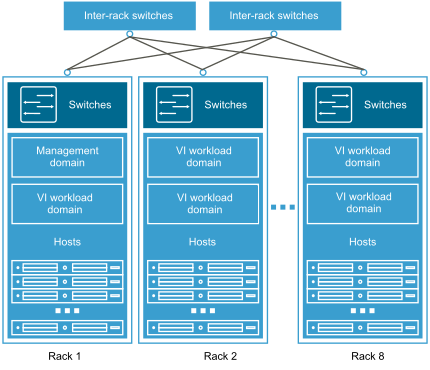
\includegraphics[width=0.75\textwidth]{imaxes/conceptosPrevios/arquitect_standarCF.png}
  \caption{Esquema del modelo de arquitectura estándar.}
  \label{fig:modelostandard}
\end{figure}
\FloatBarrier
%%%%%%%%%%%%%%%%%%%%%
%%  CONOLIDADO
\subsubsection{Modelo consolidado}
Este modelo se despliega cuando el entorno esta formado por menos de siete nodos. En este modelo, \underline{Virtual Infrastructure Domain} y \underline{Management Domain} están situados en el mismo clúster vSphere, y en caso de que se añadan más nodos al clúster, este modelo se puede convertir en un modelo estándar. Ambos dominios se mantienen aislados gracias a sus respectivos almacenes de recursos[Fig. \ref{fig:modeloconsolidated}].

\begin{figure}[h!]
  \centering
  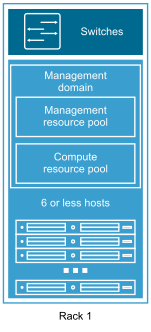
\includegraphics[width=0.25\textwidth]{imaxes/conceptosPrevios/modelConsolidated.png}
  \caption{Esquema del modelo de arquitectura consolidado.}
  \label{fig:modeloconsolidated}
\end{figure}
\FloatBarrier

%%% CLOUD BUILDER
\subsection{Cloud Foundation Builder VM Support}
\label{subsec:cloudBuilder}
El despliegue de la plataforma Cloud Foundation se realiza través de una máquina virtual llamada Cloud Foundation Builder. Esta máquina recoge la configuración que se indica en la hoja de parámetros, los valida, , despliega y configura el \underline{Management Domain}. Al final del proceso, transfiere el inventario y el control del sistema al componente SDDC Manager y esta máquina virtual puede ser eliminada.\\
\underline{Requisitos mínimos} de Cloud Foundation Builder VM:
\begin{itemize}
    \item \textbf{CPU}: 4vCPUs
    \item \textbf{Memoria}: 4 GB
    \item \textbf{Almacenamiento}: 350 GB
    \item \textbf{Conectividad}: acceso a la red de gestión para acceder a cada nodo, al servidor DNS y al servidor NTP.
\end{itemize}

\subsection{Red, almacenamiento y servicios necesarios para el despliegue}

\subsubsection{Servicios internos}
\label{subsubsec:servInterno}
Durante el despliegue Cloud Foundation, hay servicios y puertos deben estar habilitados en cada nodo ESXi para Cloud Foundation Builder (Fig. \ref{fig:puertosCB}) y SDDC Manager (Fig. \ref{fig:puertosSDDC}) puedan acceder a todos los componentes.

\begin{figure}[h!]
  \centering
  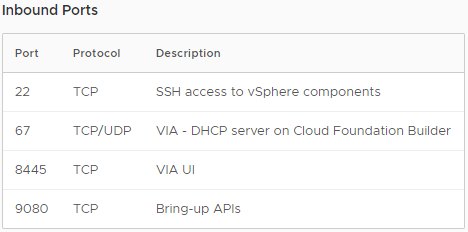
\includegraphics[width=0.7\textwidth]{imaxes/conceptosPrevios/puertosentradaCB.png}
  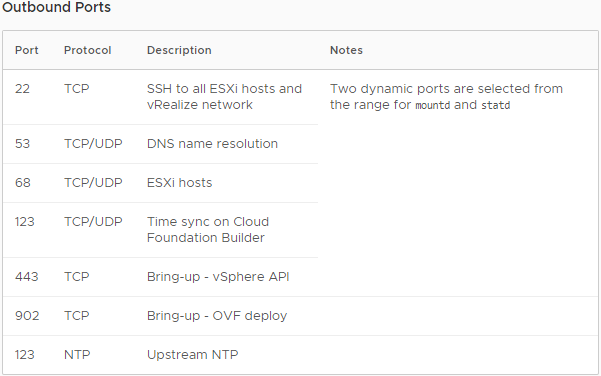
\includegraphics[width=0.7\textwidth]{imaxes/conceptosPrevios/puertossalidaCB.png}
  \caption{Servicios y puertos de entrada y salida habilitados para Cloud Foundation Builder.}
  \label{fig:puertosCB}
\end{figure}

\begin{figure}[h!]
  \centering
  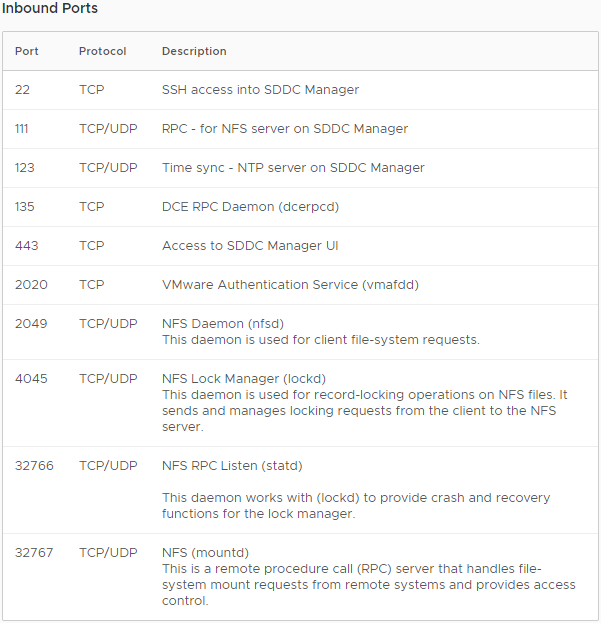
\includegraphics[width=0.7\textwidth]{imaxes/conceptosPrevios/puertosentradaSDDC.png}
  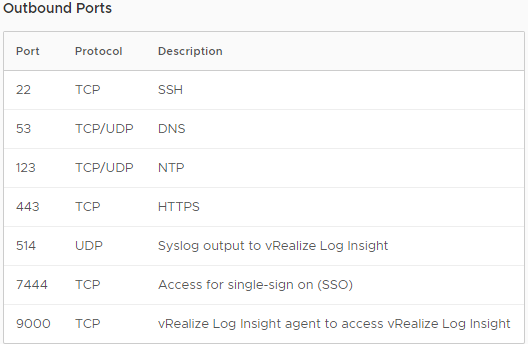
\includegraphics[width=0.7\textwidth]{imaxes/conceptosPrevios/puertossalidaSDDC.png}
  \caption{Servicios y puertos de entrada y salida habilitados para SDDC Manager.}
  \label{fig:puertosSDDC}
\end{figure}

%%%%%%%%%%%%%%%%%%%%%%%%%%%%%%%%%%%%%%%%%%%%%%%%%%%%%%%%%%%%%%%%%%%%%%%%
\iffalse
\begin{itemize}
\item Cloud Builder:
    \begin{itemize}
        \item Entrada:
            \begin{itemize}
                \item SSH: 22, TCP
                \item VIA - Servidor DHCP en Cloud Foundation Builder: 67, TCP/UDP
                \item VIA - Interfaz de Usuario: 8445, TCP
                \item APIs para controlar los componentes: 9080, TCP
            \end{itemize}
        \item Salida:
            \begin{itemize}
                \item SSH: 22, TCP
                \item DNS: 53, TCP/UDP
                \item Hosts ESXi: 68, TCP/UDP
                \item NTP: 123, TCP/UDP
                \item API para iniciar vSphere: 443, TCP
                \item Despliegue de archivos OVF: 902, TCP
            \end{itemize}
    \end{itemize}
\item SDDC Manager:
        \begin{itemize}
        \item Entrada:
            \begin{itemize}
                \item SSH: 22, TCP
                \item RPC para servidor NFS: 111, TCP/UDP
                \item NTP: 123, TCP/UDP
                \item DCE RPC: 135, TCP
                \item Interfaz de Usuario: 443, TCP
                \item Servicio de Autenticación: 2020, TCP
                \item Demonio NFS (nfsd): 2049, TCP/UDP
                \item NFS Lock Manager (lockd): 4045, TCP/UDP
                \item NFS RPC (statd): 32766, TCP/UDP
                \item NFS (mountd): 32767 , TCP/UDP
            \end{itemize}
        \item Salida:
            \begin{itemize}
                \item SSH: 22, TCP
                \item DNS: 53, TCP/UDP
                \item HTTPS: 443, TCP
                \item NTP: 123, TCP/UDP
                \item Syslog hacia vRealize Log Insight: 514, UDP
                \item Acceso Single-Sign On: 7444, TCP
                \item Agente vRealize Log Insight: 9000, TCP
            \end{itemize}
    \end{itemize}
\end{itemize}
\fi

%%%%%%%%%%%%%%%%%%%%%%%%%%%%%%%%%%%%%%%%%%%%%%%%%%%%%%%%%%%%%%%%%%%%%%%%%%%%%
\FloatBarrier

\subsubsection{Servicios externos}
\label{subsubsec:servExterno}
En este apartado se describen aquellos servicios necesarios para el despliegue de VMware Cloud Foundation
\begin{itemize}
    \item Dynamic Host Configuration Protocol (DHCP): Permite configurar automáticamente cada puerto VMkernel de un nodo con IPv4. 
    \item Domain Name Server (DNS): Un servidor DNS debe estar disponible para todos los componentes desde el momento de despliegue. También se debe especificar el nombre del dominio. Con esto los componentes pueden obtener tanto el nombre como la dirección IP de un elemento en la red. NTP, Platform Services Controller, instancias de vCenter Server, instancias de NSX Manager, vRealize Log Insight.
    \item Network Time Protocol (NTP): Permite la sincronizar el tiempo en todos los nodos de la infraestructura. Durante el despliegue se debe especificar la dirección IP de al menos un servidor NTP.
\end{itemize}
Se puede encontrar más información sobre otros servicios opcionales en el siguiente \href{https://docs.vmware.com/en/VMware-Cloud-Foundation/3.9/com.vmware.vcf.planprep.doc_39/GUID-F022BD3C-F11C-4EE6-83EA-ABE016E7A9B9.htm}{enlace}.
\FloatBarrier

%%%%% RED 
\subsubsection{Red física}
\label{subsubsec:redFisica}
La red física debe admitir las siguientes características:
\begin{itemize}
    \item VLAN: etiquetado de redes VLAN (802.1Q)
    \item Jumbo Frames: MTU mínimo igual a 1600, aunque se recomienda que sea igual a 9000.
\end{itemize}

\subsubsection{Red lógica}
\label{subsubsec:redLogicaCF}
Antes del despliegue es necesario especificar varias redes que más tarde Cloud Foundation usará para automatizar la configuración de puertos \ref{Word:vmkernel} cuando se añade un nuevo host al entorno o se crea un VI Domain. Estas redes son  una dedicada al servicio \underline{vSAN}, otra dedicada a \underline{vMotion}, ota de dedicada a la gestión de los componentes y otra dedicada al tráfico de las máquinas virtuales. Los datos a especificar son la etiqueta VLAN, MTU, IP de la red, máscara, gateway y el rango de direcciones IP. Una vez creadas solo se puede modificar el rango de direcciones IP.\\
Es importante utilizar VLANs e IPs ya que es en lo que se basa Cloud Foundation para aislar cada tipo de tráfico de la infraestructura. La cantidad de subredes necesarias depende del número de Workload Domains que se creen, número de clusters y otros componentes opcionales.

\subsubsection{Almacenamiento}
Según la documentación de vSAN, cada host ESXi del entorno debe tener como mínimo un grupo de discos. Un nodo puede tener hasta cinco grupos de discos, dentro de los cuales debe haber al menos un disco de caché y un disco de capacidad. Cada grupo de discos puede contener hasta siete discos de capacidad.
En cuanto al tipo de disco que se debe utilizar, los discos de caché deben ser SSD y los discos de capacidad pueden ser SSD o HDD, según el modelo que se quiera implementar (All-Flash o híbrido).

%%%%%%%%%%%%%%%%%%%%%%%%%%%%%%%%%%%%%%%

\iffalse
\subsection{Nombres y direcciones IP}
Cloud Foundation requiere especificar el nombre que se le da a cada componente y su r
Durante el despliegue hay que especificar el nombre de cada componente y su dirección IP. Estos componentes son los servicios externos, los componentes internos de Cloud Foundation como SDDC Manager, Platform Services Controller, vCenter Server, cada nodo ESXi, cada instancia de NSX y de vRealze Log Insight.
\fi


\iffalse
a
\subsection{Instancias de los componentes}
Para cada workload domain que se crea, SDDC Manager genera una serie de instancias de cada componente tanto en Management Domain como en cada Virtual Infraestructure Domain. Estas instancias son:
\subsubsection{Management Domain}
Una instancia de vCenter Server. Para la gestión de la red de este dominio, despliega una instancia de NSX Manager(centraliza la gestión de la red, aporta APIs para crear configurar y monitorizar cada componente de NSX como los switches lógicos o los servicios que operan en el gateway de salida de la red) y tres instancias de NSX Controller (gestiona el vSwitch distribuído y el enrutamiento del tráfico, controlando todos los vswitches de la red y manteniendo información sobre todas las VM, nodos, vSwitches y VXLANs. Para la gestiión de logs, se instala 
\fi
